\chapter{Aplicaciones} \label{Aplicaciones }

\section{Introducción}\label{intro_aplicaciones}

En el estudio de las matemáticas, uno encuentra resultados teóricos que son realmente fascinantes. Muchas veces, estos resultados fueron motivados por problemas prácticos. Solo por mencionar algunos de estos resultados, tendríamos el Teorema de Pitágoras y la ley de gravitación universal.\\
Además, está el estudio de esos números extraños que, en el siglo XVI, Rafael Bombelli los llamaba \capertura cantidad  salvaje'' y establecía las reglas de cálculo en su Álgebra. No fue sino hasta que Descartes los llamo \capertura números imaginarios'' y, posteriormente, Leonhard Euler introdujo la notación $i =\sqrt{-1}$, la cual ha aparecido en las ecuaciones de la mecánica cuántica y la transformada de Fourier.\\
Es por ello que, en este pequeño capítulo, presentamos algunos de los ejemplos donde podemos aplicar la teoría de los mapeos conformes a problemas físicos. 
\section{Flujo de fluidos}
Iniciamos esta sección presentando algunos conceptos clave que utilizaremos en el futuro. Es importante destacar que, para simplificar nuestra discusión, nos enfocaremos principalmente en el flujo de fluidos ideales.\\
Consideremos  un flujo de fluido ideal con el campo vectorial de velocidad
\[
	\textbf{v}=\left[\begin{array}{c}
		u(x,y)\\
		v(x,y)
	\end{array}\right]
\]
en el punto \[
\textbf{x}=\left[\begin{array}{c}
	x\\
	y\end{array}\right]
\]
donde $\textbf{v(x)}$ denota la velocidad instantánea del fluido en el punto $\textbf{x}\in \Omega\subset \R^{2}$. Diremos que el flujo es incompresible , es decir, el volumen del líquido no cambia si y sólo si 
\begin{equation}\label{ec3-1}
	\nabla \cdot \textbf{v} =\dpartial{u}{x}+\dpartial{u}{y}=0.
\end{equation}
Por otro lado, diremos que el fluido es irrotacional si

\begin{equation}\label{ec3-2}
	\nabla \times \textbf{v} =\dpartial{v}{x}-\dpartial{v}{y}=0.
\end{equation}
Un flujo diremos que es un flujo de fluido ideal si es incompresible e irrotacional. La mayoría de los líquidos y los gases se comportan como flujos ideales.\\
Note que las ecuaciones (\ref{ec3-1})-(\ref{ec3-1}) son casi idénticas a las ecuaciones de Cauchy-Riemann.\\ 
\noindent Tenemos el siguiente teorema
\begin{teor}
	El campo vectorial de velocidad $\textbf{v}=[u(x,y)\;\;\; v(x,y)]^{T}$ induce un flujo de fluido ideal si y sólo si
	\begin{equation}\label{ec3-3}
		f(z)=u(x,y)-iv(x,y),
	\end{equation}
	es una función analítica en $z=x+iy$.\endproof
\end{teor}
Note que los componentes $u$ y $-v$ del campo vectorial de velocidad para los flujos de fluidos ideales son necesariamente conjugados armónicos. La función $f(z)$ es conocida como la velocidad compleja del flujo de fluido. Bajo tal flujo, las partículas del fluido siguen las trayectorias $z(t) = x(t)+iy(t)$ obtenidas integrando el sistema de ecuaciones diferenciales ordinarias.
\begin{equation}\label{ec3-4}
	\derivada{x}{t}=u(x,y),\; \; \; \derivada{y}{t}=v(x,y),
\end{equation}
o en forma compleja 

\begin{equation}\label{ec3-5}
	\derivada{z}{t}=\overline{f(z)},
\end{equation}
donde las curvas parametrizadas por la solución $z(t)$ se conocen como líneas de corriente del flujo de fluido. Si la velocidad compleja $f(z_0)$ en un punto $z_0$ desaparece, entonces la solución $z(t) = z_0$ de la ecuación (\ref{ec3-5}) es constante y el punto $z_0$ es un punto de estancamiento del flujo.\\
En lo que respecta a Mathematica, estaremos utilizando el comando \textbf{ComplexVectorPlot}. 

\begin{Ejem}
	Sea $f(z)=1$. El vector velocidad $\textbf{v}=[1\;\;\;0]^{T}$. Entonces $\derivada{z}{t}=1$ ya que $\derivada{x}{t}=1$ y $\derivada{t}{t}=0$. Resolviendo $\derivada{z}{t}=1$ se obtiene $z(t)=t+z_0$, que Representa un flujo uniforme horizontal que se manifiesta a través de líneas rectas paralelas al eje real.\endproof
	\begin{mmaCell}{Input}
		ComplexVectorPlot[1, {z, -3 - 3 I, 3 + 3 I}]
	\end{mmaCell}
	\begin{mmaCell}[moregraphics={moreig={scale=0.3}}]{Output}
		\mmaFrac{ \mmaGraphics{37.png}}{}
	\end{mmaCell}
\end{Ejem}
\begin{Ejem}
	Sea $f(z)=c=a+bi$. Resolviendo $\derivada{z}{t}=\overline{c}=a-ib$, se tienen que $z(t)=\overline{c}t+z_0$. Las líneas de corriente son paralelas a las rectas inclinadas formando un ángulo $\theta=\operatorname{arg}(\overline{c})=\operatorname{arg}(c)$ al eje real. A continuación se muestra usando $a=3$ y $b=4$
	\begin{mmaCell}{Input}
		ComplexVectorPlot[3 + 4*I, {z, -3 - 3 I, 3 + 3 I}]
	\end{mmaCell}
	\begin{mmaCell}[moregraphics={moreig={scale=0.3}}]{Output}
		\mmaFrac{ \mmaGraphics{38.png}}{}
	\end{mmaCell}
\end{Ejem}


Supongamos ahora que la velocidad compleja $f(z)$ admite una antiderivada compleja, es decir, una
función analítica compleja $g(z)$ tal que 
\begin{equation}\label{ec3-6}
	g(z)=\phi(x,y)+i\psi(x,y),
\end{equation}
donde $\derivada{g}{z}=f(z)$.\\
Luego, de las ecuaciones de Cauchy-Riemann se sigue que
\[
\derivada{g}{z}=\dpartial{\phi}{x}-i\dpartial{\phi}{y}=u-iv \implies \dpartial{\phi}{x}=u,\; \dpartial{\phi}{y}=v.
\]
Entonces, $\nabla\phi=\textbf{v}$, y $\phi(x,y)=\operatorname{Re}\{g(x)\}$ define un potencial de velocidad del flujo de fluido. Por lo tanto, la función $g(z)$ es conocida como la función potencial compleja para el campo de velocidades dado. Luego $ \phi(x, y)$ es una función analítica y armónica que satisface la ecuación de Laplace $\nabla^{2}\phi= 0$. Por el contrario, cualquier función armónica puede considerarse como el potencial para algún flujo de fluido, donde la velocidad real del flujo es su gradiente $\textbf{v} = \nabla\phi$, representando así un flujo de fluido ideal. La función armónica $\phi(x, y)$ se conoce como función de corriente; esta cumple con la ecuación de Laplace, y las funciones de potencial y corriente están relacionadas a través de las ecuaciones de Cauchy-Riemann.
\begin{equation}\label{ec3-7}
	\dpartial{\phi}{x}=u=\dpartial{\psi}{y},\;\;\; \dpartial{\phi}{y}=v=-\dpartial{\psi}{x}.
\end{equation}
Los conjuntos de nivel del potencial de velocidad, definidos por $\{\phi(x,y)=c,\;c\in\R\}$, se conocen como curvas equipotenciales. El potencial de velocidad $\textbf{v}=\nabla \phi\neq 0$ es normal a las curvas equipotenciales. Notemos que, $\textbf{v}=\nabla \phi$ también es tangente a las curvas de nivel $\{\phi(x,y)=d\}$ de su función armónica conjugada. Pero $\textbf{v}$ al ser el campo de velocidad, es tangente a las líneas de corriente debidas a las partículas del fluido. Por lo que, estos dos sistemas de curvas deben ser iguales. Por lo tanto, las curvas de nivel de las líneas de corriente del flujo, y el conjunto de curvas equipotenciales $\{\phi=c\}$ y el conjunto de líneas de corriente $\{\psi=d\}$  son dos familias mutuamente ortogonales de curvas planas.  

\begin{Ejem}[Flujo alrededor de un disco]
	Considere la función potencial compleja
	$$g(z)=z+\dfrac{1}{z}=\left(x+\dfrac{x}{x^2+y^2}\right)+i\left(y-\dfrac{y}{x^2+y^2}\right),$$
	donde las partes real e imaginaria son soluciones de las ecuación de Laplace en dos dimensiones.  el  campo de flujo complejo correspondiente es 
	$$f(z)=\derivada{g}{z}=1-\dfrac{1}{z^2}=1-\dfrac{x^2-y^2}{(x^2+y^2)^2}+i\dfrac{2xy}{(x^2+y^2)}.$$
	Los puntos $z=\pm 1$ son puntos de estancamiento del flujo, y $z=0$ es una singularidad. Por lo tanto, el fluido que se mueve a lo largo del eje real positivo  se acerca al punto de estancamiento $z=-1$ cuando $t\rightarrow \infty$. Notemos que las líneas de corriente $\phi(x,y)=y-\dfrac{y}{x^2+y^2}=d$ se vuelven horizontales a medida que más se alejen del origen, es flujo es similar al un flujo horizontal uniforme, de izquierda a derecha, con velocidad compleja unitaria $f(z)=1$.
	
	Las curvas de nivel para $d = 0$ consisten en el círculo unitario $|z| = 1$ en el eje real. En particular, el círculo unitario consta de dos líneas de corriente semicirculares junto con dos puntos de estancamiento.
	La velocidad del flujo $\textbf{v} = \nabla\phi$ es tangente en todas partes al círculo unitario y, por lo tanto, satisface la condición $\mathbf{v}\cdot\mathbf{n}=0$ a lo largo de la frontera $|z|=1$.
	  
	Nuestro resultado en Mathematica 
	\begin{mmaCell}{Input}
		ComplexVectorPlot[z + (z/(z*z)), \{z, -3 - 3 I, 3 + 3 I\}, \\RegionFunction -> Function[\{z, f\}, Abs[z] > 1]]
	\end{mmaCell}
	\begin{mmaCell}[moregraphics={moreig={scale=0.3}}]{Output}
		\mmaFrac{ \mmaGraphics{39.png}}{}
	\end{mmaCell}
\end{Ejem}

\section{Transferencia de calor}
Los problemas de transferencia de calor pueden ser resueltos tanto por métodos analíticos como métodos usando mapeos conformes. Las trasformaciones conformes que se utilizan son
\begin{itemize}
	\item $z=\sen w$,
	\item $w=-i\dfrac{z-1}{z+1}$,
	\item $T=z^2$,
	\item  $w=i\log T=2i\log z$,
\end{itemize}
La ecuación de calor es 
\begin{equation}\label{ec3-8}
	u_t=ku_{xx}
\end{equation}
donde $k$ se le conoce como coeficiente de difusividad térmica.\\
A continuación se presentan algunos ejemplos que comúnmente se resuelven en un curso ordinario de ecuaciones diferenciales parciales (EDP) usando métodos analíticos.
\begin{Ejem}
	Considere la ecuación de calor 
	$$u_t=ku_{xx},\;\;\; -\infty<x<\infty,\;\;\;t>0$$
	Esta ecuación tiene los siguientes conjuntos de soluciones 
	\begin{itemize}
		\item [(i)] $u_0(x,t)=Ax+B$, donde $a$ y $B$ son constantes arbitrarias, y
		\item [(ii)]  $u_\lambda(x,t)=\cosh(\lambda x)e^{{k\lambda^2t}}$, donde $\lambda\in\R^{+}$.
	\end{itemize}
	Notemos que para cualquier $t$ fijo, 
	$$\lim_{x\rightarrow\pm\infty}u_\lambda(x,t)=+\infty$$
	Como estas soluciones no están acotadas cuando $x\rightarrow\pm\infty$, estas no son aceptables para problemas físicos. Si se requiere que la solución $u$ sea acotada en el infinito tanto en $x$ como en $t$, debemos  de establecer las siguientes condiciones 
	\[
	\begin{array}{ccc}
		\ds\lim_{x\rightarrow\pm\infty}u(x,t)<\infty,&&\ds\lim_{t\rightarrow\infty}u(x,y)<\infty,
	\end{array}
	\]
	así como la condición inicial $u(x,0)=f(x)$, $-\infty<x<\infty$, donde $f(x)$ es una función acotada para todo $x$.\endproof
\end{Ejem}
\begin{Ejem}
	Considere la ecuación de calor 
	$$u_t=ku_{xx},\;\;\; 0<x<l$$
	sujeta a las condiciones iniciales y de frontera
	\[
	\begin{array}{cccc}
		u(0,t)=0=u(l,t),& t>0,&u(x,0)=f(x),&0<x<l,
	\end{array}
	\]
	donde $f\in C^{1}$. En términos físicos, este problema representa la conducción de calor en una varilla cuando sus extremos se mantienen a temperatura cero mientras que la temperatura inicial $u$ en cualquier punto de la varilla esta dada por $f(x)$. Usando el método de separación de variables y las condiciones anteriores, la solución es
	$$u(x,t)=\sum_{n=1}^{\infty}C_n\sen \left(\dfrac{n\pi x}{l}\right)e^{\frac{-kn^2 \pi^2 t}{l^2}},$$
	donde $$C_n=\dfrac{2}{l}\int_{0}^{l}f(x)\sen\left(\dfrac{n\pi x}{l}\right)dx,\;\;\;n=1,2,3,\ldots$$\endproof
\end{Ejem}
\begin{Ejem}
	Considere la ecuación de calor 
	$$u_t=u_{xx},\;\;\; 0<x<1$$
	sujeta a las condiciones iniciales y de frontera
	\[
	\begin{array}{ccccc}
		u(0,t)=1,&u(1,t)=0,&t>0& u(x,0)=0,&0<x<1
	\end{array}
	\]
	En este ejemplo, primero encontremos una solución particular, para ello podemos tomar el caso de estado estacionario, donde la ecuación se convierte en $\tilde{u_{xx}}=0$, la cual al integrar dos veces se obtiene la solución general
	$$\tilde{u}(x)=c_1x+c_2.$$
	Luego, usando las condiciones de frontera $\tilde{u}(0)=1$, $\tilde{u}(1)=0$ obtenemos la solución en el estado estacionario $$\tilde{u}(x)=1-x.$$
	A continuación, formulamos un problema homogéneo escribiendo $u(x, t)$ como una suma de la solución de estado estacionario $\tilde{u}(x)$ y un término transitorio $v(x,t)$, es decir, $u(x,t)=\tilde{u}(x)+v(x,t)$ o 
	$$v(x,t)=u(x,t)-\tilde{u}(x).$$
	Sustituyendo esta ecuación en el problema original se obtiene 
	$$v_t=v_{xx},$$
	donde las condiciones de frontera e iniciales se reducen a 
	\[
	\begin{array}{c}
		v(0,t)=u(0,t)-\tilde{u}(0)=0\\
		v(1,t)=u(1,t)-\tilde{u}(1)=0\\
		v(x,0)=u(x,0)-\tilde{u}(x)=x-1
	\end{array}
	\]
	Resolviendo esta EDP se obtiene 
	$$v(x,t)=\sum_{n=1}^{\infty}C_ne^{-n^2\pi^2t}\sen n\pi x,$$
	donde $$C_n=2\int_{0}^{1}(x-1)\sen n\pi x dx=-\dfrac{2}{n\pi}.$$
	Luego $$v(x,t)=-\dfrac{2}{\pi}\sum_{n=1}^{\infty}\dfrac{1}{n}e^{-n^2\pi^2t}\sen n\pi x,$$
	Por lo tanto 
	$$u(x,t)=1-x-\dfrac{2}{\pi}\sum_{n=1}^{\infty}\dfrac{1}{n}e^{-n^2\pi^2t}\sen n\pi x.$$\endproof
\end{Ejem}
Los siguientes ejemplos se resuelven usando transformaciones conformes 
\begin{Ejem}
	Considere el caso de la distribución de temperatura en las regiones semicirculares superior e inferior del disco unitario con la temperatura en la frontera dada por
	\[
	u=\left\{
	\begin{array}{ccc}
		20^{\circ}&\mbox{si}& \theta\in(0,\pi)\\
		0^{\circ}&\mbox{si}&\theta\in (-\pi,0)
	\end{array}
	\right.
	\]
	Para encontrar la temperatura en los puntos $z=0$ y $z=\dfrac{1}{2}$, usaremos la función $$\zeta=i\dfrac{1-z}{1+z},$$ esta función mapea la región $|z|<1$ en el semiplano superior del plano $\zeta$, de modo que la frontera superior del disco unitario se mapee en el eje positivo $\xi$ mientras que la frontera inferior se mapee en  el eje negativo $\xi$ (vea la Figura \ref{fig:40}).
	\begin{figure}
		\centering
		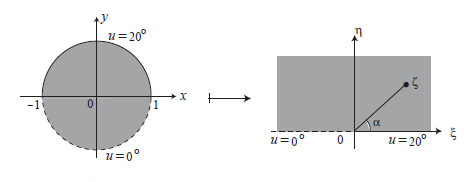
\includegraphics[width=0.7\linewidth]{img/40}
		\caption{Mapeo del círculo al semiplano superior}
		\label{fig:40}
	\end{figure}
	Entonces la distribución de la temperatura en el plano $\zeta$ esta dada por $u=A\alpha+B$, donde $\alpha=\arctan(\eta/\xi)$, donde $\arctan(\eta/\xi) \in [0,\pi]$, de las condiciones de frontera se tiene $B=20$ y $A=-20/\pi$, por lo tanto,
	\begin{equation}\label{ec3-9}
		u=-\dfrac{20}{\pi}\arctan(\eta/\xi)+20,
	\end{equation}
	si usamos la función $\zeta=-i\dfrac{z-1}{z+1}$ obtenemos 
	$$\xi+i\eta=-i\dfrac{x-1+iy}{x+1+iy}=-i\dfrac{x^2+y^2-1+2iy}{(x+1)^2+y^2}.$$
	Igualando las partes reales e imaginarias se tiene que 
	\begin{equation}\label{ec3-10}
		\xi=\dfrac{2y}{(x+1)^2+y^2},\;\;\;\eta=\dfrac{1-x^2-y^2}{(x+1)^{2}+y^2}.
	\end{equation}
	Sustituyendo (\ref{ec3-10}) en (\ref{ec3-9}) obtenemos las distribución de la temperatura
	\begin{equation}\label{ec3-11}
		u(x,y)=-\dfrac{20}{\pi}\arctan\left(\dfrac{1-x^2-y^2}{2y}\right)+20.
	\end{equation}
	Entonces, la temperatura en $z=0$ es 
	$$u(0,0)=-\dfrac{20}{\pi}\arctan(\infty)+20=-\dfrac{20}{\pi}\dfrac{\pi}{2}+20=10^{\circ}$$
	ya que $\tan(\pi/2)=\infty$, y la temperatura en $(0,1/2)$ es
	$$u\left(0,\dfrac{1}{2}\right)=-\dfrac{20}{\pi}\arctan\left(\dfrac{3}{4}\right)+20\approx16.9^{\circ}.$$\endproof
\end{Ejem}

\section{Campo electromagnético}
Imagine un alambre conductor ortogonal al plano $z$ en el origen, sobre el cual se distribuye uniformemente una carga eléctrica de densidad $q$ unidades de carga en el alambre. El potencial eléctrico generado por este cable es $u = -2q \log r$, y el potencial complejo es
\begin{equation}\label{ec3-12}
	f(z)=2q\log z,
\end{equation}
esto debido a que en general, una linea de carga $q$ por unidad de longitud esta sujeta a la fuerza $q\mathbf{E}$ por unidad de longitud, donde $\mathbf{E}$ es el vector que describe la intensidad del campo eléctrico, el cual esta definido por 
\begin{equation}\label{ec3-13}
	\textbf{E}=-\nabla u, \;\; \mbox{ y }\;\; \textbf{E}=-\overline{f'(z)}
\end{equation} 
\begin{Ejem}
	Sea $q_1$ una carga por unidad de longitud en $z=0$ y sea $q_2$ otra carga por unidad de longitud en $z=1$. Entonces de (\ref{ec3-11}) el potencial complejo esta dado por la suma de los potenciales debido a las fuentes en $z=0$ y $z=1$, es decir,
	\begin{equation}\label{ec3-14}
		f(z)=-2q_1\log z-2q_2\log (z-1).
	\end{equation}
	Dado que el potencial $u=\operatorname{Re}(f(z))$, tenemos que 
	\[
	\begin{array}{ccl}
		u&=&-2q_1\ln |z|-2q_2\ln|z-1|\\
		&=&-2q_1\ln\sqrt{x^2+y^2}-2q_2\ln\sqrt{(x-1)^2+y^2}\\
		&=&-q_1\ln(x^2+y^2)-q_2\ln((x-1)^2+y^2).
	\end{array}
	\]
	De (\ref{ec3-13}) tenemos que 
	$$\mathbf{E}=-\overline{f'(z)}=-(\overline{-2(q_1\ln|z_1|+q_2\ln|z-1|)'})=2\left(\overline{q_1\dfrac{1}{z}+q_2\dfrac{1}{z-1}}\right)=\dfrac{2q_1}{\bar{z}}+\dfrac{2q_2}{\bar{z}-1}$$
	
\end{Ejem}
Cuando $$\operatorname{Im}(f(z))=v=c,$$ donde $c$ es constante, las líneas $v=c$ son llamadas lineas de fuerza y el vector $\mathbf{E}$ es tangente a estas líneas.\\
En el ejemplo anterior, si $q_1=q_2=q-2q\ln|z(z-1)|-2qi\operatorname{arg}\{z(z-1)\}$ y como $\operatorname{arg}\{z(z-1)\}=\dfrac{2xy-y}{x^2-y^2-x}$, la parte imaginaria del potencial complejo es dada por 
$$v(x,y)=-2q\arctan\dfrac{2xy-y}{x^2-y^2-x},$$
y entonces, las líneas de fuera, definidas por $v=c$, son dadas por 
$$\dfrac{2xy-y}{x^2-y^2-x}=\tan\left(-\dfrac{c}{2q}\right)=C$$
donde $C$ es una constante.\\ Las líneas de fuerza $v=c$, en los puntos $z=\pm 1$ se muestran en la a continuación.
\begin{mmaCell}{Input}
	 Show[StreamPlot[\{(2*x*y - y)/(x^2 + y^2 - x), 1.0\},\\\{x, -10, 10\}, \{y, -10, 10\}],ListPlot[\{\{-1, 0\}, \{1, 0\}\}, \\PlotStyle -> Red]]
\end{mmaCell}

\begin{mmaCell}[moregraphics={moreig={scale=0.3}}]{Output}
	\mmaFrac{ \mmaGraphics{41.png}}{}
\end{mmaCell}

\printbibliography[heading=bibintoc]